\chapter{Results from previous models}

\section{\citet{bib:maher-1982}}

\begin{figure}[H]
    \centering
    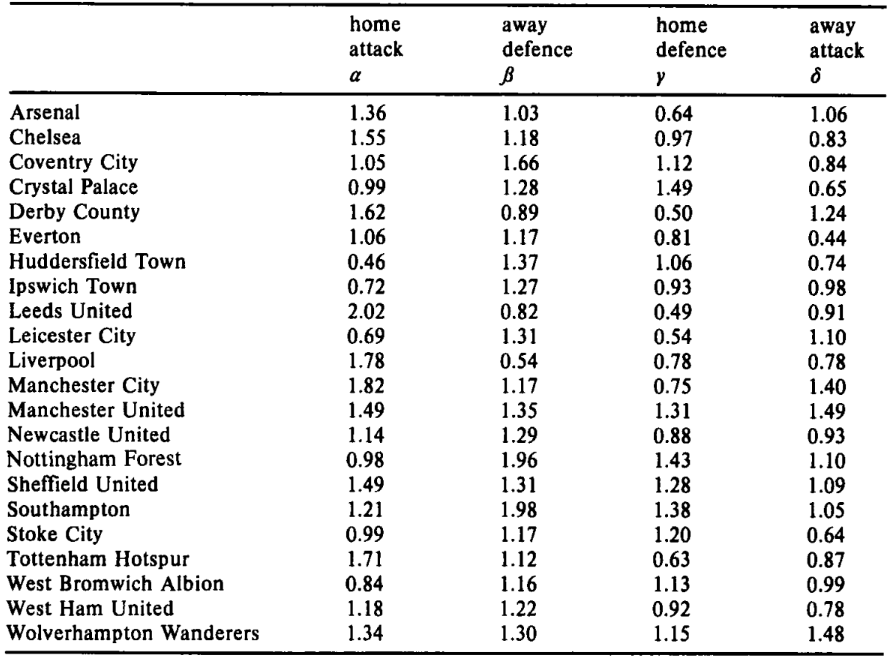
\includegraphics[width=\textwidth]{results/maher-strengths.png}
    \caption{Maximum likelihood estimates of the parameters for the English Division 1 1971-1972. Taken from \citet{bib:maher-1982}.}
    \label{fig:app-maher-strengths}
\end{figure}

\begin{figure}[H]
    \centering
    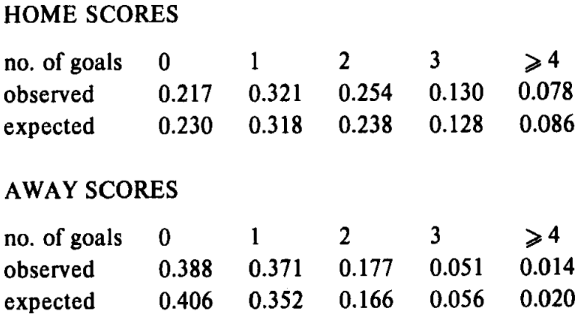
\includegraphics[width=\textwidth]{results/maher-double-frequencies.png}
    \caption{Comparison of expected and observed number of goals scored for home and away teams for the English Division 1 1971-1972. Taken from \citet{bib:maher-1982}.}
    \label{fig:app-maher-double-frequencies}
\end{figure}

\begin{figure}[H]
    \centering
    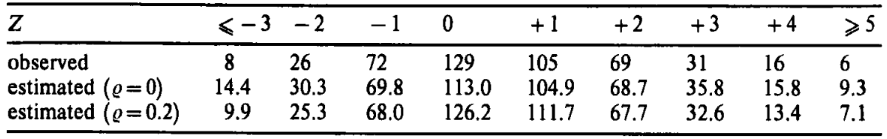
\includegraphics[width=\textwidth]{results/maher-bivariate-frequencies.png}
    \caption{Observed and estimated frequencies for Z, the goal difference, for the English Division 1 1971-1972 using different values for $\varrho$. Taken from \citet{bib:maher-1982}.}
    \label{fig:app-maher-bivariate-frequencies}
\end{figure}


\section{\citet{bib:karlis-ntzoufras-2003}}

\begin{figure}[H]
    \centering
    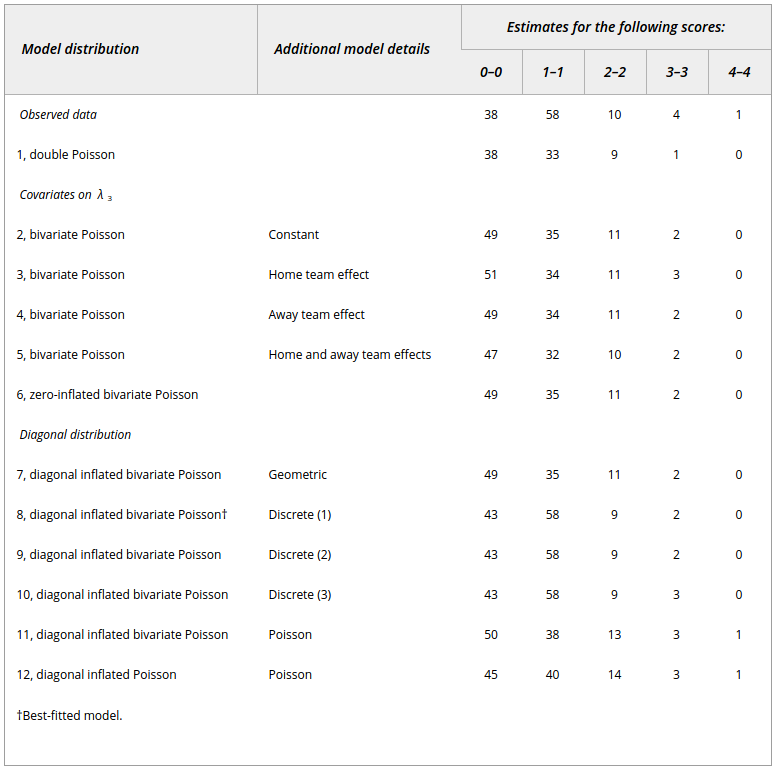
\includegraphics[width=\textwidth]{results/karlis-ntzoufras-2003-results.png}
    \caption{The estimates by different versions of the model from \citet{bib:karlis-ntzoufras-2003}. Taken from \citet{bib:karlis-ntzoufras-2003}.}
    \label{fig:app-karlis-ntzoufras-2003-results}
\end{figure}


\section{\citet{bib:koopman-lit-2015}}

\begin{figure}[H]
    \centering
    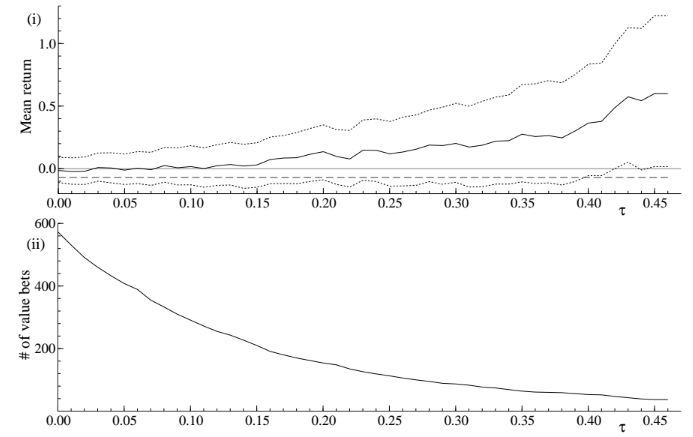
\includegraphics[width=\textwidth]{results/koopman-lit-threshold-levels.png}
    \caption{(i) The average return from betting on match outcomes in the English Premier League 2010-2012 using different values for $\tau$. Plotted together with $90\%$ bootstrap confidence intervals. (ii) The number of feasible bets for different values of $\tau$. Taken from \citet{bib:koopman-lit-2015}.}
    \label{fig:app-koopman-lit-threshold-levels}
\end{figure}


\section{\citet{bib:rue-salvesen-2000}}

\begin{figure}[H]
    \centering
    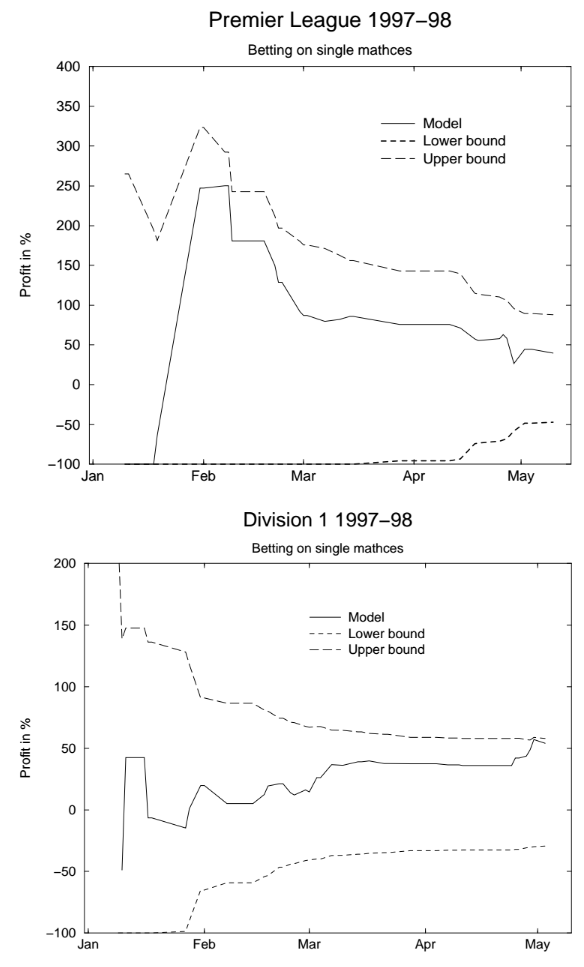
\includegraphics[width=0.8\textwidth]{results/rue-salvesen-profits.png}
    \caption{The observed profit in the simulated betting experiments for the English Premier League 1997-1998. Taken from \citet{bib:rue-salvesen-2000}.}
    \label{fig:app-rue-salvesen-profits}
\end{figure}


\section{\citet{bib:hvattum-arntzen-2010}}

\begin{figure}[H]
    \centering
    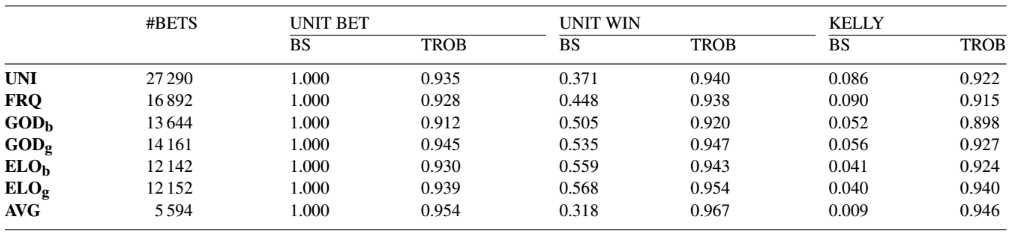
\includegraphics[width=\textwidth]{results/hvattum-arntzen-2010-profits.png}
    \caption{Average bet size (BS) and total return on bets (TROB) based on simulated betting on 14,927 matches from the English league system, using seven different betting strategies. Here, UNIT BET represents Fixed bet, UNIT WIN Fixed return, and Kelly the Kelly ratio strategy. Taken from \citet{bib:hvattum-arntzen-2010}.}
    \label{fig:app-hvattum-arntzen-2010-profits}
\end{figure}


\section{\citet{bib:constantinou-fenton-neil-2012}}

\begin{figure}[H]
    \centering
    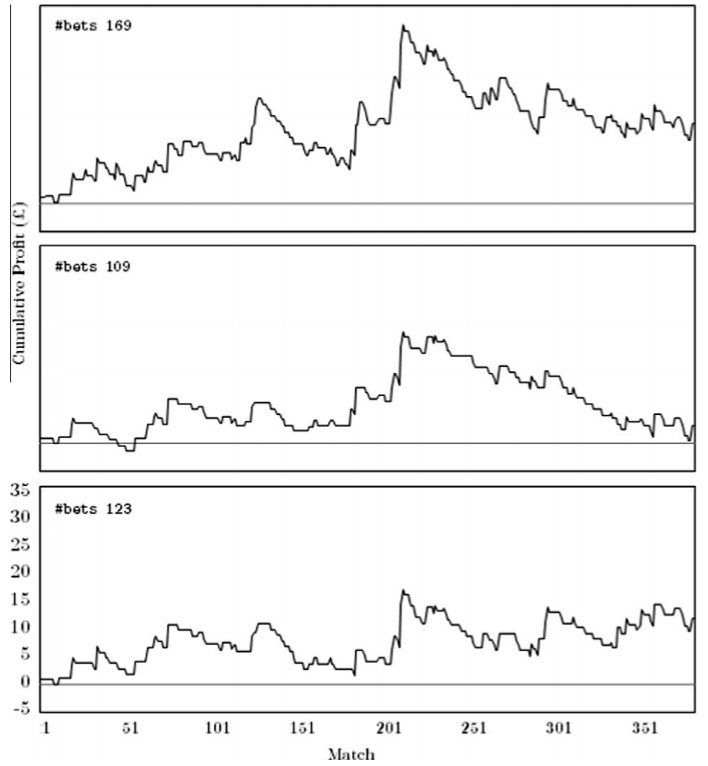
\includegraphics[width=\textwidth]{results/constantinou-fenton-neil-2012-profits.png}
    \caption{Cumulative profits observed when simulating the Unit bet strategy at discrepancy levels of $\geq 5\%$ against (a) $f_{maxB}$, (b) $f_{meanB}$, and (c) $f_{WH}$. Taken from \citet{bib:constantinou-fenton-neil-2012}.}
    \label{fig:app-constantinou-fenton-neil-2012-profits}
\end{figure}

\begin{figure}[H]
    \centering
    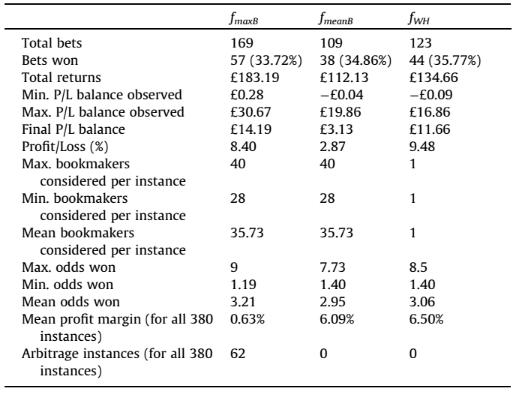
\includegraphics[width=\textwidth]{results/constantinou-fenton-neil-2012-bets.png}
    \caption{Betting simulation stats against (a) $f_{maxB}$, (b) $f_{meanB}$, and (c) $f_{WH}$ at discrepancy levels of $\geq 5\%$. Taken from \citet{bib:constantinou-fenton-neil-2012}.}
    \label{fig:app-constantinou-fenton-neil-2012-bets}
\end{figure}